\section{Project Management}\label{sec:project-management}
% Tracking todos with GitHub issues
The project was managed with an iterative and incremental process, organised using weekly sprints that were planned and tracked via the ZenHub\cite{_zenhub_????} tool for GitHub. Zenhub adds progress tracking and analytics for GitHub projects as well as project management features such as Kanban style boards.

\begin{wrapfigure}[12]{r}{0.4\textwidth}
  \vspace{-2mm}
  \centering
  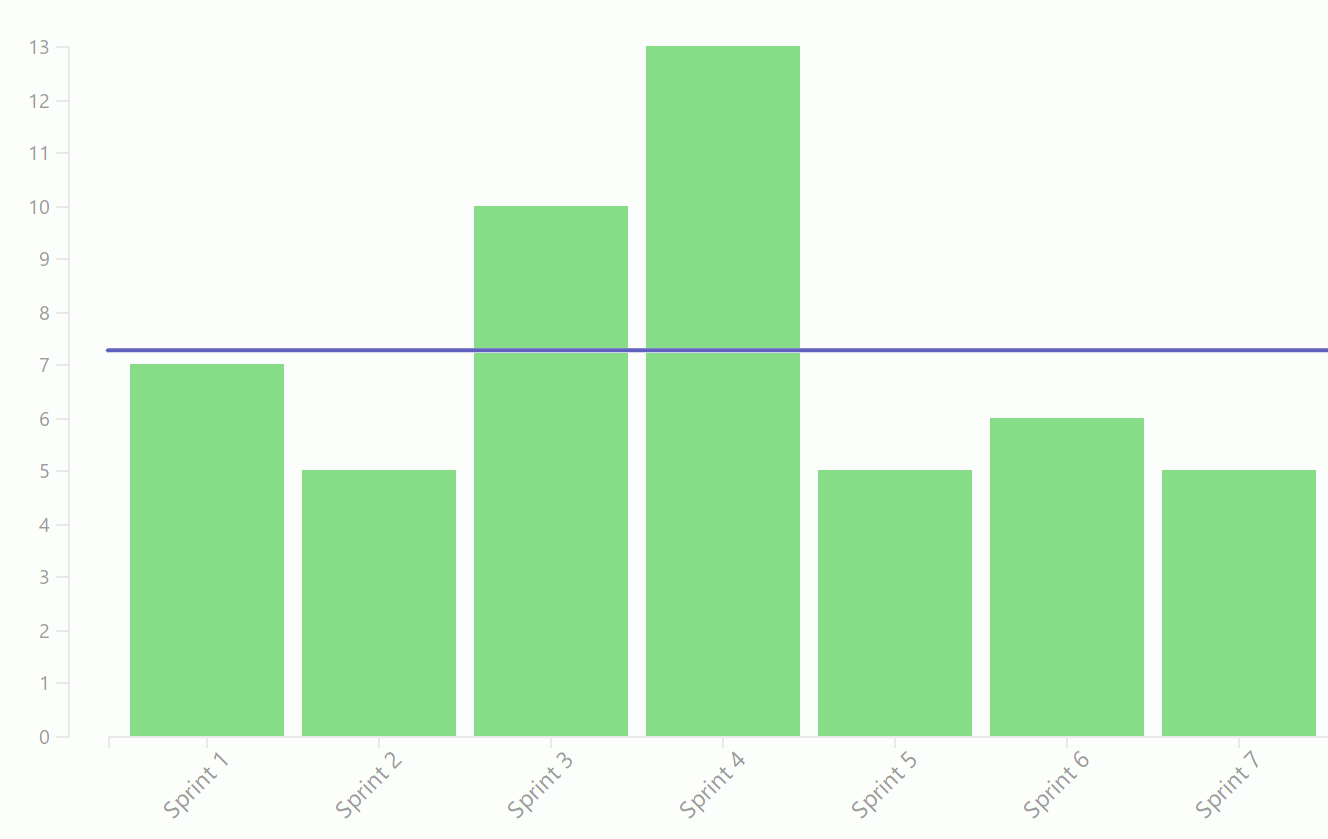
\includegraphics[width=\linewidth]{img/velocity-tracking.png}
  \caption{ZenHub sprint velocity tracking for the first seven weeks of the project}\label{fig:velocity-tracking}
\end{wrapfigure}

All tasks for the project had a formal issue created for them on GitHub so that their progress and details could be tracked. Each issue could be tagged with any of the following labels:
\begin{itemize}[noitemsep]
  \item bug
  \item design
  \item documentation
  \item enhancement
  \item feature
  \item research
  \item testing
\end{itemize}

An issue would also be given a complexity value that could be chosen from the fibonacci sequence, these should typically not be above 5, otherwise the issue should likely be split into more manageable tasks. The fibonacci sequence is used as a popular Scrum method to reflect the uncertainty that comes with estimating more complex items, since the values grow rapidly.

Issues follow the template of requiring:
\begin{enumerate}[noitemsep]
  \item a user story
  \item acceptance criteria
  \item a definition of completeness
\end{enumerate}
This is not a hard requirement as a structure but it does ensure that required detail is included for features and enhancements.


Sprints were managed on a weekly basis, tasks would be chosen from the list of issues and assigned to a GitHub milestone representing a sprint. Using milestones, we were able to see the progress of a sprint as issues were closed.
The ZenHub tool being used allows for a lot of estimation and tracking of progress in the project. Sprints are shown as a bar chart in the ``Velocity Tracking'' feature. Completed sprints are given a score that is the total number of complexity points for all issues solved within the time period. This allowed for us to estimate what could be completed based on previous data. Figure~\ref{fig:velocity-tracking} shows the first few weeks of the project in the velocity tracking feature.

ZenHub also allowed us to track several other useful statistics in the project such as a ``burndown'' graph showing ideal and actual progress towards completing all points in a sprint.
Kanban style project management boards were used to manage the issues created to track tasks, this can be seen in Figure~\ref{fig:kanban-board}. This means that issues move between different categories on a ``board'' indicating their status. Several different categories were created for tasks to move through, listed below:
\begin{description}[noitemsep]
  \item New Issues: Issues that have not been reviewed
  \item Icebox: Issues that will not be worked on in the near future
  \item Backlog: Issues that can be worked on
  \item Sprint Backlog: Issues to be completed in the current sprint
  \item In Progress: Issues currently being worked on
  \item Closed: Completed issues
\end{description}

\begin{figure}[ht]
  \centering
  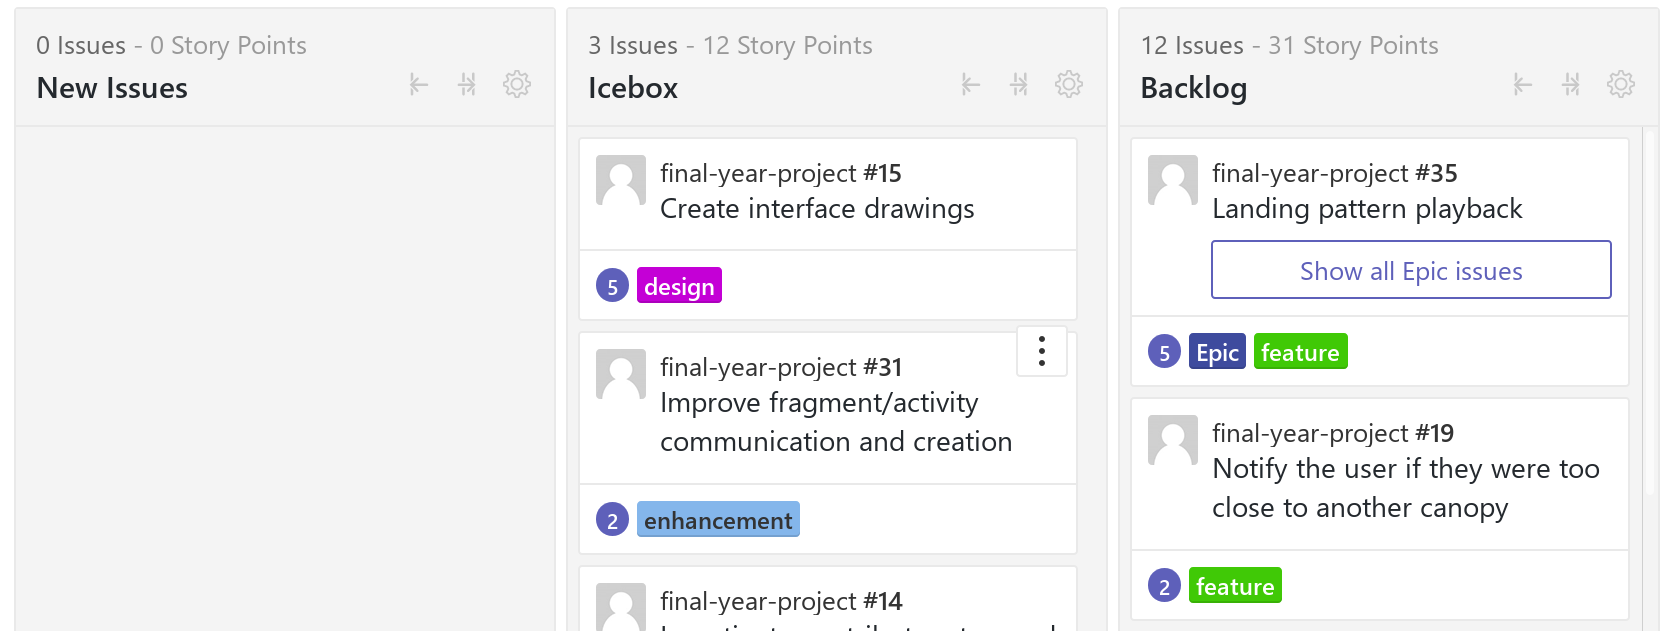
\includegraphics[width=\linewidth]{img/issue-board.png}
  \caption{Some ZenHub Kanban style boards used in the project}\label{fig:kanban-board}
\end{figure}

The methods for management of the project were appropriate and useful, ensuring that all tasks were tracked, detailed and planned. The use of ZenHub's additional features and statistics for the repository ensured that goals were realistic and achievable.
